%Travail technique
	%But?
	%Overview (Mockups, workflows)
	%Algorithme
	%Architecture et Design
	%Implémentation (langage et librairies utilisés)
	%Utilisation (screenshots, etc)


\chapter{Travail technique}
	\thispagestyle{document}
	
\section{Principe}
\label{sec:principe}

\par Le principe est d'utiliser les suites de tests d'un projet comme spécifications de celui-ci. Chacune d'entre elles est liée à une méthode pas encore implementée. Lors de l'exécution des tests, toutes les variables accessibles depuis la méthode ciblée seront collectées, ce sont les sorties. De plus, les assertions contenu dans le test permettent de définir les valeurs attendu par l'exécution de la méthode ciblée, ce sont les sorties. Il est ensuite possible de combiner de nombreuse manières les entrées avec des opérateurs afin d'essayer d'arriver à la sortie. Si une tel combinaison existe, la méthode est donc synthétisable, sinon il faudra réitérer après avoir synthétiser d'autres méthodes, augmentant le nombre d'entrées.


\section{Overview}
\label{sec:overview}

\subsection{Ciblage}
\label{subsec:ciblage}
\par Les méthodes testées doivent être référencés de manières explicites dans les tests associés. Une convention a été mise en place, le développeur doit ensuite la respecter lors de l'écriture des spécifications. La figure \ref{fig:ciblage} représente un exemple de ciblage. À la différences des annotations, cette convention ne demande pas d'ajouter de nouvelle dépendances à un projet car elle utilise simplement la documentation.

\begin{figure}[H]
\begin{lstlisting}
/**
 * @link mon.package.MaClass#MaMethod(type.param1, type.param2)
 */
\end{lstlisting}
\caption{Exemple de ciblage utilisé à l'aide de la Javadoc}
\label{fig:ciblage}
\end{figure}

\subsection{Entrées}
\label{subsec:collecte_entree}
\par La collecte des entrées est effectuée par DynaMoth. Une position dans le code source doit être définie lorsque le synthétiseur est appelé. Cette position correspond à la dernière ligne de la méthode ciblée. DynaMoth utilise ensuite une API\footnote{\url{https://fr.wikipedia.org/wiki/Interface_de_programmation}} de débogage pour placer un point d'arrêt. Il collecte ensuite toutes les valeurs accessibles ou possible lors de chaque exécution de la position : les variables, les attributs et même les appels de méthodes. Des constantes peuvent également être ajoutées.

\subsection{Sorties}
\label{subsec:collecte_sorties}
\par La collecte des sorties s'effectue en modifiant les tests et en les exécutants. La transformation représentée dans la figure \ref{fig:collect_sorties} a pour but de récupérer les valeurs attendues par les assertions pour ensuite les envoyer à DynaMoth. Les sorties sont évalué et collecté de manières dynamiques.

\begin{figure}[H]
\begin{lstlisting}
methodTest :
+   collect(methodeCible.signature, methodTest.signature, sortie1)
    assertion(sortie1, methodeCible(param1))
+   collect(methodeCible.signature, methodTest.signature, sortie1)
    assertion(sortie2, methodeCible(param1))
\end{lstlisting}
\caption{Exemple de transformation pour récupérer les sorties}
\label{fig:collect_sorties}
\end{figure}

\subsection{Combinaisons}
\label{subsec:combinaisons}

\par Une fois les entrées et sorties collectées, il faut les faire correspondre. Pour chaque exécution de la position ciblée, il faut trouver une relation entre toutes les entrées et la sortie. Si cette relation n'est pas direct, DynaMoth essaye de combiner les entrées avec des opérateurs pour agrandir l'ensemble des possibilités. Si aucune relation existe, il recommence récursivement jusqu'à trouver une relation, ou atteindre un \textit{timeout} paramètrable. La table \ref{fig:operateurs} représente les opérateurs utilisées par DynaMoth.

\begin{table}[H]
\centering
\begin{tabular}{|c|c|}
\hline
Unaire & ! ++ $--$ \\
Binaire & \&\& $|$ $|$ == != $<$= $<$ + $-$ * / \% \\
\hline

\end{tabular}
\caption{Les opérateurs utilisés par DynaMoth}
\label{fig:operateurs}
\end{table}
 

\section{Implementation}
\label{sec:implementation}

\par ??? est implementé en Java, pour les différentes transformation et instrumentation de code source, il utilise Spoon\footnote{\url{http://spoon.gforge.inria.fr/}}. Les spécifications sous forme de tests sont également écrite en Java, à l'aide du framework JUnit\footnote{\url{http://junit.org/}}. Comme énoncé en \ref{subsec:ciblage}, le ciblage de méthode utilise la Javadoc et \textit{@link}. ??? utilise également Maven Invoker API\footnote{\url{https://maven.apache.org/shared/maven-invoker/}}, afin de démarrer différent \textit{goals} sur le projets en cours d'analyse.


\subsection{Injection}

\par La phase de collecte des sorties expliquée en \ref{subsec:collecte_sorties} s'effectue de la manière suivante. Les tests sont modifiées à l'aide Spoon pour récupérer les valeurs attendues par les assertions. Or, puisque ces tests seront exécuter à l'aide de Maven Invoker API, le context de ??? ne sera pas accessible. Pour résoudre se problème, ??? injecte également du code dans le projet en cours de modification, ainsi qu'un \textit{Runner} personnalisé. La collecte se fera donc dans le context du projet en cours d'intrumentation. À la fin de l'exécution des tests, le \textit{Runner} sérialisera les sorties dans un fichier. Il ne restera plus qu'à ??? de les récupérer une fois le \textit{goal} maven terminé. La figure \ref{fig:workflow_collectes_sorties} représente le workflow lors de la phase de collecte des sorties.

\begin{figure}[H]
\begin{center}

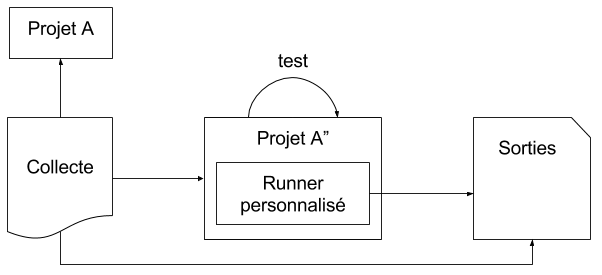
\includegraphics[scale=.7]{Workflow_output_collector.png}

\end{center}
\caption{Workflow d'exécution lors de la collecte des sorties}
\label{fig:workflow_collectes_sorties}
\end{figure}

\subsection{Test}

\par TRY/CATCH TO PRESERVED ORIGINAL BEHAVIOUR

\par Le framework JUnit fonctionne le manière suivante, lors qu'une assertion échoue à l'intérieur d'un test, elle soulève une exception. Cependant, lors d'un tel comportement, les assertions suivantes ne seront pas exécutées et donc pas collectées. Afin collecter toutes les sorties, la transformation appliquée insert également des \textit{try/catch} pour ne pas stopper l'exécution du test. Une exception est soulevée à la fin du test, uniquement si l'une des assertions a échoué. La figure \ref{fig:collect_sorties_try_catch} reprend l'exemple énoncé en \ref{subsec:collecte_sorties} en appliquant cette transformation supplémentaire.

\begin{figure}[H]
\begin{lstlisting}
public void test() :
+ hasException=false
+ try
+   collect(methodeCible.signature, methodTest.signature, sortie1)
    assertion(sortie1, methodeCible(param1))
+ catch AssertionError
+   hasException=true
+ try
+   collect(methodeCible.signature, methodTest.signature, sortie2)
    assertion(sortie2, methodeCible(param1))
+ catch AssertionError
+   hasException=true
+ assertion(hasException, false)
\end{lstlisting}
\caption{Exemple de transformation spécifique à JUnit pour récupérer les sorties}
\label{fig:collect_sorties_try_catch}
\end{figure}

\section{Scope}
\label{sec:scope}

\par ??? se limite uniquement aux méthodes ayant un type de retour, les méthodes de type \textit{void} ne peuvent pas être synthétisées. De plus, la phase de collecte des sorties expliquée en \ref{subsec:collecte_sorties} ne permet pas de récupérer une sortie de type exception lorsqu'elle est spécifiée dans l'annotation \textit{@Test}.





\section{Utilisation}

\begin{figure}[H]

\begin{verbatim}
Usage: OLS_Repair
	    -s, --source-path           path_program
	    -m, --maven-home-path       path_maven_home
   [-c, --constant              one_constant_to_add]*
   [-t, --time-out-collection   time in second]
   [-d, --time-out-dynamoth     time in second]
   [-o, --override]
   [-v, --verbose]
\end{verbatim}

\end{figure}
	

	
		
		
		